%\documentclass{buIE47xbooklet}
%\documentclass[print]{buIE47xbooklet}
\documentclass[nocoverpage]{buIE47xbooklet}
% You can give the following options inside [...] before {...}
% nocoverpage: removes the cover page. cover page contains project short name and team number.
% print      : removes the hyperlink colors

% Use in paper preamble \addtitlepagetop, \addtitlepagebottom, \addtitlepageleft, \addtitlepageright with negative lengths
% (e.g., \addtitlepagetop{-1cm}) to enlarge titlepage margins if necessary (e.g., to fit all material into one page)


% Proje ismi
\TRprojectname{Sezonsal ve Rassal Talep Altında Dinamik Üretim Planlama}

% Project name
\ENGprojectname{Dynamic Production Planning Under
Seasonal and Stochastic Demand}

% Company name
\TRcompany{Nesco Gıda}

% Team numbers
\teamno{21}

% Project short name
\projectshortcode{TCOTZ}  

% Team members
\teammembers{%
	Derin Aktürk,
	Osmantan Beşikci,
	Melike Karalar,\\
	Berke Kemahlı,
	Kenan Arda Köymen,
	Bahadır Maral,
    Deniz Yaşar
}

% Industrial advisors
% Use optional form \IA[team]{...} if you have two or more IAs
\IA{%
	Nazlı Esen Ummansu \\
	Kurucu/CEO 
}

% Academic advisor(s)
% Use optional form \AA[team]{...} if you have two or more AAs
\AA{%
	Doç. Dr. Özlem Çavuş İyigün\\
	Endüstri Mühendisliği Bölümü
}

% Uncomment the next command and change information to acknowledge TÜBİTAK support you may have received. 
%\ack{This project was supported by TÜBİTAK BİDEB 2209/B Program under Grant 1234C123456789.}

% Özet
\TRabstract{%
Bubble tea alanında üretim yapan ve Nesco Gıda'nın alt markası olan BobaCo, belirsiz ve sezonsal talepler ve üretim kapasitesi kısıtları nedeniyle müşteri talebini etkin biçimde karşılamakta zorlanmaktadır. Bu projenin amacı, şirketin mevcut kapasitesi ile bu talebi daha verimli karşılayabilmesi için bir üretim ve envanter karar destek sisteminin geliştirilmesidir. Ele alınan sistemin hesaplama zorlukları nedeniyle, rassal yaklaşım ile döner çevren mantığını birleştiren bir sezgisel çözüm yöntemi önerilmiştir. Bu yöntem, iki farklı planlama ufkunda çalışan matematiksel modellerin hiyerarşik biçimde bütünleştirilmesiyle sağlanmıştır. Önerilen yaklaşım ve geliştirilen karar destek sistemi, fazla mesai gereksinimi ve birikmiş sipariş ölçülerinde iyileştirme sağlayan yüksek kaliteli ve uygulanabilir üretim planları üretmektedir.
}

% Anahtar Sözcükler
\TRkeywords{
Hiyerarşik Üretim Planlaması, Döner Çevren Yeniden Eniyileme, Rassal Programlama, Uzun Dönem Planlama, Mevsimsel ve Belirsiz Talep, Önceden Stok Oluşturma, Karar Destek Sistemi
}


% Abstract
\ENGabstract{%
BobaCo, a bubble tea producer and sub-brand of Nesco Gıda, faces difficulties in meeting customer demand due to uncertain seasonal patterns and production capacity constraints. This project aims to develop a production and inventory decision support system to enable the company to meet this demand more efficiently under its existing capacity structure. Due to the computational complexity of the system, a heuristic solution approach that combines stochastic modeling with a rolling horizon methodology is proposed. This approach is built on the hierarchical integration of mathematical models operating over two different planning horizons. The proposed approach and decision support system generate production plans that improve overtime and backlog metrics. 
}

% Keywords
\ENGkeywords{
Hierarchical Production Planning, Rolling Horizon, Stochastic Programming, Long-Term Aggregate Planning, Seasonal and Uncertain Demand, Inventory Build-Ahead, Decision Support System
}

% Bibliography file name
\bibfilename{booklet.bib}

% Team photo file name
\teamphoto{figures/group_photo.png}


\begin{document}

\section{Company Description}
NESCO is a domestically managed food and beverage company founded in 2016 and headquartered in Ankara, Türkiye, operating with an innovative approach in the industry. From raw material sourcing and product development to production, worldwide sales, and distribution, NESCO manages all major functions of its value chain in-house, allowing it to maintain product quality and respond flexibly to customer needs. It supplies more than 3,500 companies in Turkey and exports to over 30 countries, serving both domestic HORECA and international B2B customers. Its fastest-growing brand, BobaCo, is among the first brands to manufacture bubble tea on an industrial scale in Türkiye, with 25 distinct popping boba flavors~\citep{BobaCo}. The products are primarily supplied through a B2B model to cafés, coffee chains, restaurants, hotels, and beverage brands, while some formats are also offered in retail packaging.

\section{System Analysis and Problem Definition}

\subsection{System Analysis}
The BobaCo production system consists of four interrelated products: Plastic Tub Boba, Semi-Finished Boba in Tub, Cup Bubble Tea, and Can Bubble Tea. Plastic Tub Boba is sold directly as a finished product, mainly for the domestic market, whereas Semi-Finished Boba in Tub serves only as an input in the production of Cup and Can Bubble Tea. Production is organized on two lines\index{constraint!line assignment}. The first line produces Plastic Tubs and Semi-Finished Boba, which follow the same production flow but differ in formulation, making them operationally similar yet distinct for planning. The second line produces Cup and Can Bubble Tea, but due to pasteurization constraints, these two products cannot be produced on the same day. In addition, once a line is assigned to a product, it cannot switch to another on the same day, so each line can process at most one product per day.

\subsection{Problem Definition}
In previous years, the company faced pronounced demand peaks during the summer season. However, meeting this demand was difficult due to limited production capacity. Although product shelf life allows inventory to be carried over multiple months, limited storage space in the previous facility prevented the company from building inventory ahead. With the transition to a new facility, storage limitations have eased, creating the opportunity to build inventory in advance\index{inventory!build-ahead}. This shift makes it essential to develop a planning approach that coordinates production capacity\index{constraint!production capacity} and inventory decisions over time. The key challenge is to balance holding and backlogging costs while maintaining production feasibility for both raw materials and finished goods under seasonal\index{forecasting!seasonal demand} and uncertain\index{forecasting!uncertain demand} demand. The company prepares its production plan and schedule semi-manually by evaluating market insights, past experiences, and previous demand data. Since demand, particularly in the domestic market, is both seasonal and difficult to predict precisely, a reliable and mathematically grounded decision support system is needed to support production planning under uncertainty. The objective of this decision support system is to generate a production plan that determines the appropriate production and stocking levels of different product types, minimizing holding and backlogging costs during the high-demand season while satisfying system requirements. Accordingly, the problem extends beyond simple capacity allocation and requires coordinated production and inventory decisions under seasonal and uncertain demand.
\section{Proposed Solution Approach}

\subsection{Critical Assumptions}
There were several critical assumptions made in order to create the models effectively and efficiently. Semi-finished Boba and Tub Boba are considered as different products. Each production line can produce at most one product type per day. Backlogging is allowed in the system to preserve feasibility; however, delays within two weeks are treated as non-critical, whereas delays beyond two weeks are considered more severe and are penalized more heavily to reflect the risk of order cancellations. 

\subsection{Major Constraints}
Production lines cannot switch between products within the same day. There are two production lines: the first line produces Plastic Tub Boba and Semi-Finished Boba, while the second line produces Cup and Can Bubble Tea. Total production in each period is limited by the available workdays, excluding overtime. Since Semi-Finished Boba is not directly demanded, it is used as an input in the production of Cup and Can products. Semi-Finished Boba may also be stored for future use. The remaining products are directly demanded by end customers and may also be stored. Storage area of the facility is limited, meaning that the total area occupied by stored products cannot exceed the available capacity. In addition, raw material availability is constrained by procurement lead times and minimum order quantities\index{constraint!minimum order quantity}. Backlogging\index{terms!backlog} is allowed, but delays exceeding 12 days\index{terms!critical backlog} are treated as critical through an additional penalty structure.

\subsection{Objectives}

The primary objective is to determine a long-term production and inventory strategy that minimizes holding and backlog costs while ensuring adequate inventory coverage for the high-demand season. Since backlog costs are higher than inventory holding costs, the planning approach is designed to discourage excessive delay while avoiding unnecessary inventory buildup. 

\subsection{Conceptual Model}



The main model is formulated as a multi-period production and inventory planning structure that represents how products flow through production, inventory, and demand fulfillment over time. Within this structure, production decisions determine period-by-period output, inventory allows available stock to be carried into future periods\index{model!inventory planning}, and backlog captures unmet demand that is postponed to later periods.  

The model also captures the structural dependency among products within the system. While Plastic Tub Boba, Cup Bubble Tea, and Can Bubble Tea are directly demanded products, Semi-Finished Boba is not directly demanded and instead serves as an input for Cup and Can Bubble Tea. Accordingly, the system is represented as an integrated planning structure in which production and inventory decisions for different products must remain coordinated and consistent over the planning horizon.



\subsection{Heuristic Solution Method}

\subsubsection{Hierarchical Heuristic Approach}
The initial “full-scale” model was formulated at a daily resolution over a one-year horizon and tailored to the facility’s specific operational restrictions and characteristics to reflect the production system accurately. However, solving a fully integrated, daily, full-year model within a reasonable runtime becomes computationally challenging due to the size of the decision space. Therefore, a hierarchical heuristic\index{production planning!hierarchical} approach is adopted by decomposing the planning problem into two coordinated models: a long-term aggregate production planning model given in Appendix~\ref{app:A} and a short-term production planning model given in Appendix~\ref{app:B}, implemented with a rolling-horizon\index{production planning!rolling horizon} mechanism ~\citep{bitran1982hpp}. This hierarchical coordination between the long-term and short-term models is illustrated in Figure \ref{fig:Hierarchical_models}.

\begin{figure}[h!]
    \centering
    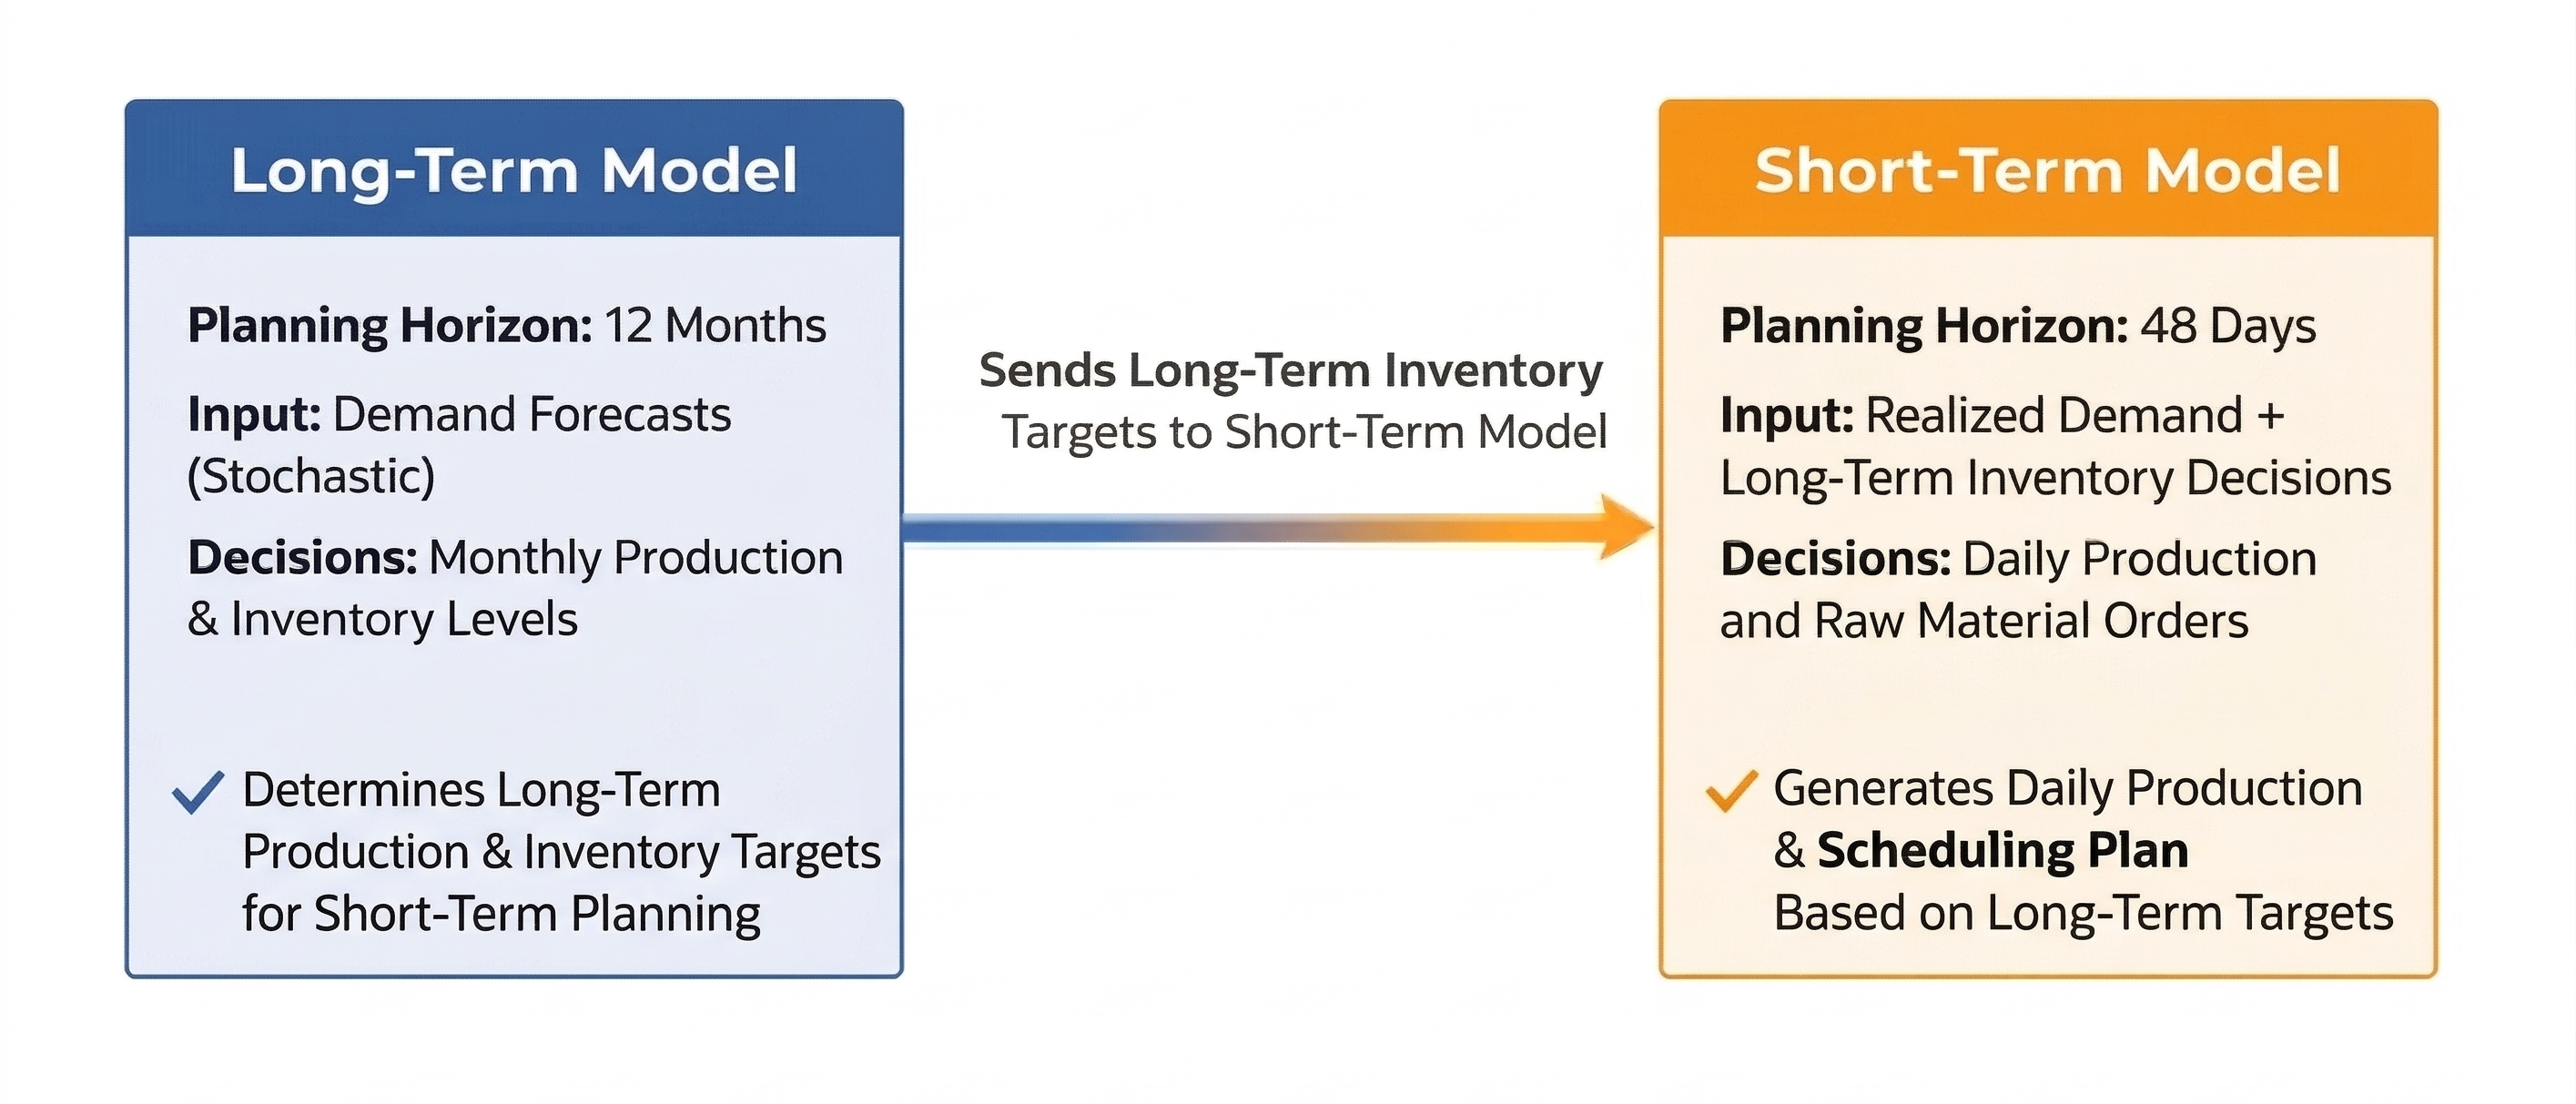
\includegraphics[width=1\linewidth]{figures/Hierarchical_models.png}
    \caption{Hierarchical Models Diagram}
    \label{fig:Hierarchical_models}
\end{figure}

\subsubsection{Stochastic Long-Term Model}
The long-term model determines strategic inventory targets over a one-year horizon at a monthly level\index{model!aggregate production planning}. It identifies in which months production should be increased to prepare for peak-season demand and sets targeted monthly inventory levels\index{production planning!monthly inventory targets}. The long-term model optimizes these targets by minimizing expected total cost, including inventory holding and backlog-related penalty components, while maintaining consistency with major system limits and planning rules ~\eqref{eq:A1}.

To account for demand uncertainty, the long-term model is formulated as a two-stage stochastic program\index{model!two-stage stochastic programming}\index{model!stochastic}, in which demand for the first two months is treated as deterministic, while demand in the remaining periods of the planning horizon is modeled as random \citep{BirgeLouveaux2011}. Based on the deviation margins provided by the company, an uncertainty band is defined around the company’s baseline forecast, and multiple demand scenarios are generated\index{terms!scenario generation} accordingly. Equal probabilities are assigned to each scenario, and the long-term model evaluates the expected total cost across the scenario set. This scenario-based formulation produces monthly inventory targets that are more resilient to uncertainty and reduces the limitations of relying on a single forecast.
\subsubsection{Short-Term Production Planning Model}
The short-term model\index{programming!mixed integer linear programming} uses the inventory decisions for the first two months obtained from the long-term model as input and translates the monthly inventory targets into operationally feasible daily decisions within an eight-week planning horizon ~\eqref{eq:B11}. In particular, it generates a detailed daily production plan that aligns with the facility’s line-level constraints and converts the higher-level inventory targets into executable production quantities, inventory updates, and short-term fulfillment decisions \eqref{eq:B2}. It also generates raw material order decisions\index{production planning!raw material ordering} to ensure material availability and maintain consistency between short-term production requirements and procurement needs \eqref{eq:B7},\eqref{eq:B8}. In this way, the proposed heuristic approach combines daily production planning in the short-term model with inventory targets generated by the long-term model, resulting in a hierarchical decision support structure that improves peak-season planning while maintaining computational and operational feasibility.
\subsubsection{Rolling-Horizon Structure}
The two models operate under a rolling-horizon structure: the long-term model is re-run on a monthly basis to refresh monthly inventory targets as new information becomes available, while the short-term model is updated weekly to produce an actionable near-term schedule. 


\section{Validation}
Using the company’s actual input data and forecast structure, the rolling-horizon decision support system produced planning patterns consistent with the company’s operational logic. In particular, during peak-demand periods, the system builds inventory ahead and later uses this inventory to control backlog. It was also observed that when forecasts are updated or available workdays decrease, the rolling-horizon structure responds quickly by revising build-ahead and production decisions, making the system more responsive to changing operating conditions. As shown in Figure \ref{fig:Pro_dem}, the model initially built inventory in anticipation of higher forecasted demand, and later reduced production when realized demand turned out to be lower than expected. This behavior is well aligned with the company’s planning needs, since the main challenge in the current system is not only meeting seasonal demand, but also reacting in a timely and structured manner to changing production conditions.

\begin{figure}[h!]
    \centering
    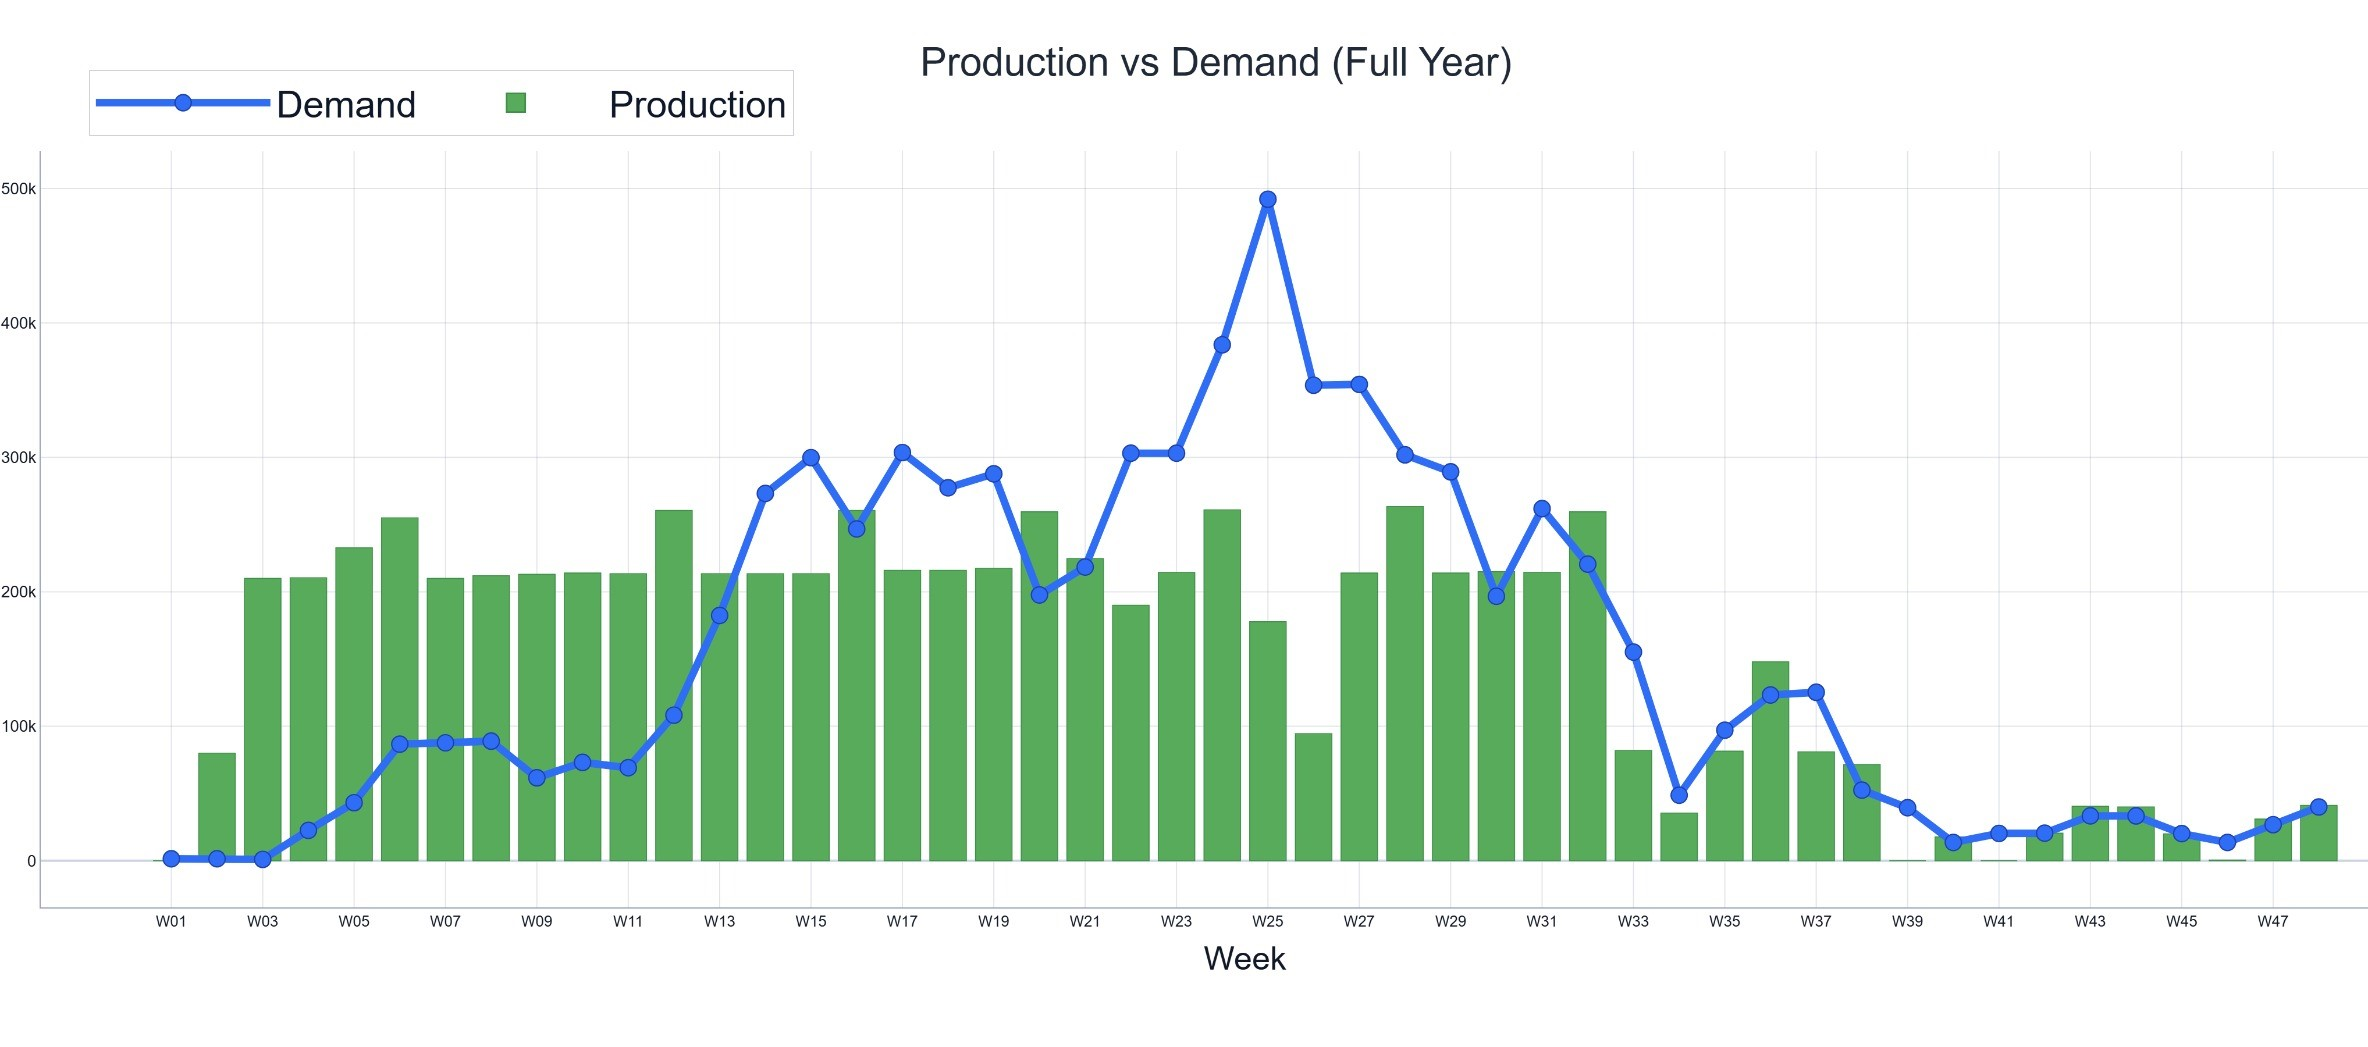
\includegraphics[width=1\linewidth]{figures/Production_demand.jpeg}
    \caption{Production and Demand Levels Throughout the Year}
    \label{fig:Pro_dem}
\end{figure}

Both the rolling-horizon structure and the stochastic long-term component contribute meaningfully to the company’s ability to prepare for future demand scenarios. While the rolling-horizon structure improves the company’s ability to respond to demand changes in a timely and consistent manner, the stochastic long-term model generates more protective inventory targets under uncertainty. In the yearly rolling-horizon implementation, this more cautious inventory policy increased the average holding-cost component by 94.2\%, while reducing the average backlog-cost component by 46.4\%. This result is consistent with the model structure, since backlog costs are very large and the stochastic model reacts to uncertainty by keeping more inventory in order to reduce the risk of future backlog. Accordingly, although the holding-cost component increases, the stochastic approach reduces the average total cost by 42.0\%. These values should be interpreted as model-based performance measures rather than direct accounting costs, but they still indicate that the stochastic policy provides a more robust balance between inventory protection and backlog risk under uncertainty.



\section{Benchmarking and Benefits}

Benchmarking analysis was conducted to compare the proposed decision support system with the company’s current planning approach under the same demand inputs. In this comparison, the current system was represented by a 45-day backward allocation rule. Since the company responds to delays exceeding 12 days through overtime usage, the benchmarking focuses on backlog risk and overtime\index{terms!overtime} dependency. The following KPIs were used in the comparison: Backlog Under Cancellation Risk\index{terms!cancellation risk}, Overtime Days, and Overtime Delivery Rate (the share of total demand that must be recovered through overtime production).

Under the original 2026 forecast, the current system required 11 overtime days and created 380,709 units of backlog under cancellation risk out of a total demand of 6,330,210 units. This corresponds to 6.01\% of total demand being under cancellation risk. Under the same forecast, the proposed system eliminated overtime need completely and produced no residual backlog.

To test the robustness of the proposed system under uncertainty, 10 demand scenarios were generated around a monthly forecast. Under these scenarios, the current system required between 17 and 37 overtime days, with an average of 28.2 days, and created 8,082,588 units of backlog under cancellation risk over a total demand of 64,721,203 units, corresponding to a weighted backlog-under-cancellation-risk ratio of 12.49\%. In contrast, the proposed system achieved zero backlog and zero overtime in 7 of the 10 scenarios. In the remaining 3 scenarios, it required just 1 overtime day and generated limited residual backlog. Overall, its average overtime requirement was 0.3 days, and its total remaining backlog was 49,330 units, corresponding to 0.08\% of total demand. A summary of the comparative performance of the current and proposed systems is presented in Table \ref{tab:benchmark_results}.
\begin{table}[h!]
\centering
\caption{Scenario-based results for the current and proposed systems}
\label{tab:benchmark_results}
\renewcommand{\arraystretch}{0.9}
\begin{tabular}{|p{5.8cm}|c|c|}
\hline
\textbf{\footnotesize Metric} & \textbf{\footnotesize Current System} & \textbf{\footnotesize Proposed System} \\ \hline
\footnotesize Average overtime days across 10 scenarios & \footnotesize 28.2 & \footnotesize 0.3 \\ \hline
\footnotesize Weighted backlog-under-cancellation-risk ratio & \footnotesize 12.49\% & \footnotesize 0.08\% \\ \hline
\footnotesize Scenarios with zero backlog and zero overtime & \footnotesize 0/10 & \footnotesize 7/10 \\ \hline
\end{tabular}
\end{table}

These findings show that the company’s current planning logic is highly sensitive to demand fluctuations and frequently requires reactive overtime to recover delayed orders. The proposed rolling-horizon decision support system performs much more robustly by building inventory ahead when necessary and limiting backlog accumulation beyond the 12-day tolerance window. Therefore, the main benefit to the company is not only a reduction in backlog risk, but also a substantial reduction in overtime dependency under both the base forecast and the generated demand scenarios. Numerically, this means that the proposed system reduces the average overtime requirement from 28.2 days to 0.3 days and achieves zero backlog and zero overtime in 7 out of 10 generated demand scenarios. 

\section{Implementation and Pilot Study}
The decision support system was integrated into the company’s weekly production planning process through a structured four-week pilot study. In coordination with company representatives, an interface was developed in line with the firm’s existing reporting practices, which facilitated adoption by planners. Figure \ref{fig:weekly_output} presents the user interface of the decision support system together with a sample weekly production schedule generated by the system. The first week was conducted under the close supervision of the project team, while the following weeks were carried out directly by the company within its regular planning routine. On a weekly basis, the tool generated recommended production quantities and raw material order decisions based on updated demand information and current operational inputs. These recommendations were reviewed every Monday for feasibility and shop-floor consistency, and the finalized plans and manual adjustments were documented in weekly decision records.

\begin{figure}[h!]
    \centering
    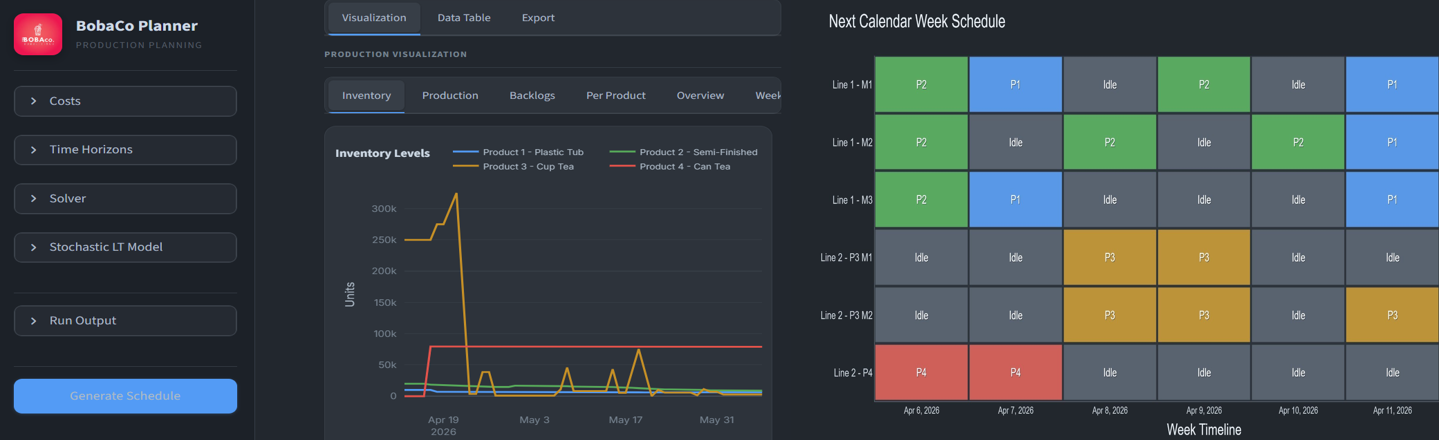
\includegraphics[width=1.04\linewidth]{figures/Ui_and_Wschedule.png}
    \caption{System interface and sample weekly schedule output.}
    \label{fig:weekly_output}
\end{figure}

The pilot study confirmed that the system could support proactive inventory build-ahead in response to forecasted peak-season demand. In particular, the system led the company to hold inventory that it had not originally planned to keep, but that was necessary to prepare for the high demand anticipated in the 2026 summer forecast. Weekly inventory quantities were recorded to monitor stock levels and their evolution throughout the pilot period. At the end of the study, the recorded decisions and inventory data indicated that the system’s outputs were compatible with weekly planning requirements and operational practice. Overall, the pilot met the company’s main expectations by demonstrating both operational practicality and the suitability of the system for regular use.

\section{Conclusion}
The project met the company’s expectations by developing a decision support system that improves production planning under seasonal and uncertain demand. The proposed structure combines hierarchical production planning, a stochastic long-term model, a short-term production planning model, and a rolling-horizon mechanism to produce plans that are both operationally feasible and responsive to changing conditions. The validation results showed that the system supports proactive inventory build-ahead and reacts quickly to forecast updates and changes in available workdays. In addition, the yearly rolling-horizon implementation results indicated that the stochastic approach provides a more robust balance between inventory protection and backlog risk under uncertainty, reducing the average total cost by 42.0\%. This relatively great improvement is mainly due to the model structure, where backlog costs are much higher than holding costs, so carrying additional inventory helps avoid much larger backlog-related losses.

The practical value of the system was also demonstrated through benchmarking and pilot use. Compared with the company’s current planning logic, the proposed approach substantially reduced overtime dependency, lowering average overtime requirement from 28.2 days to 0.3 days and achieving zero backlog and zero overtime in 7 out of 10 generated demand scenarios. In addition, the four-week pilot study showed that the system could be incorporated into the company’s weekly planning routine and could support inventory positioning for the high demand anticipated in the 2026 summer forecast. Future work may focus on improving the scenario generation structure through observations collected over longer periods, allowing demand uncertainty to be represented in an even more realistic way.





\appendix

\section{Stochastic Long-Term Model}
\label{app:A} 
{\footnotesize
\noindent\textbf{Sets:}

\vspace{0.5em}
\noindent\begin{tabular}{p{0.18\textwidth}p{0.75\textwidth}}\toprule
\textbf{Symbol} & \textbf{Explanation} \\ \midrule
$K_1$ & Set of Plastic Tub and Semi-Finished Boba products \\
$K_2$ & Set of Cup Bubble Tea and Can Bubble Tea products \\
$T$ & Set of planning periods (months), $T=\{1,\dots,12\}$ \\
$\Omega$ & Set of scenarios \\ \bottomrule
\end{tabular}
\vspace{0.8em}

\noindent\textbf{Parameters:}

\vspace{0.5em}
\noindent\begin{tabular}{p{0.24\textwidth}p{0.69\textwidth}}\toprule
\textbf{Symbol} & \textbf{Explanation} \\ \midrule
$d_{i,t}$ & Demand of product $i\in K_1 \cup K_2$ in period $t \in \{1,2\}$ \\
$d_{i,t,\omega}$ & Demand of $i\in K_1 \cup K_2$ in period $t \in \{3,\dots,12\}$ under scenario $\omega \in \Omega$ \\
$a_t$ & Number of workdays in period $t \in T$ \\
$b_i$ & Backlog cost for product $i \in K_1 \cup K_2 $ \\
$c_1$ & Daily unit capacity of production line 1 \\
$c_{2,i}$ & Daily capacity of production line 2 for product $i \in K_2$ \\
$r_i$ & Unit usage area of product $i\in K_1 \cup K_2$ \\
$u_{i2}$ & Number of product 2 used in the product $i \in \{3,4\}$ \\
$h_i$ & Holding cost of product $i\in K_1 \cup K_2$ for one unit per period \\ \bottomrule
\end{tabular}

\vspace{0.8em}
\noindent\textbf{Decision Variables:}

\vspace{0.5em}
\noindent\begin{tabular}{p{0.24\textwidth}p{0.69\textwidth}}\toprule
\textbf{Symbol} & \textbf{Explanation} \\ \midrule
$P_{i,t}$ & Production of product $i\in K_1 \cup K_2$ in period $t \in \{1,2\}$ \\
$I_{i,t}$ & Inventory of product $i\in K_1 \cup K_2$ at the end of period $t \in \{1,2\}$ \\
$B_{i,t}$ & Backlog of product $i\in K_1 \cup K_2$ in period $t \in \{1,2\}$ \\
$P_{i,t,\omega}$ & Production of $i\in K_1 \cup K_2$ in period $t \in \{3,\dots,12\} $ under scenario $\omega  \in \Omega$ \\
$I_{i,t,\omega}$ & Inventory of $i\in K_1 \cup K_2$ in period $t \in \{3,\dots,12\}$ under scenario $\omega  \in \Omega$ \\
$B_{i,t,\omega}$ & Backlog of $i\in K_1 \cup K_2$ in period $t\in \{3,\dots,12\}$ under scenario $\omega  \in \Omega$ \\ \bottomrule
\end{tabular}

\vspace{1em}
\noindent\textbf{Objective Function:}
\setlength{\jot}{2pt}
\begin{flalign}
& \begin{aligned}[t]
\min\ & \sum_{t=1}^{2}\sum_{i \in K_1 \cup K_2} \left(b_i B_{i,t} + h_i I_{i,t}\right) + \sum_{\omega \in \Omega}\sum_{t=3}^{12}\sum_{i \in K_1 \cup K_2}
p_{\omega}\left(b_i B_{i,t,\omega} + h_i I_{i,t,\omega}\right)
\end{aligned}
&& \tag{A.1}\label{eq:A1}
\end{flalign}

\noindent\textbf{Constraints:}
\vspace{0.5em}

\noindent\textit{Production Capacity Constraints:}
\setlength{\jot}{2pt}
\begin{flalign}
& \sum_{i \in K_1}\frac{P_{i,t}}{c_1} \le a_t \quad , \quad
  \sum_{i \in K_2}\frac{P_{i,t}}{c_{2,i}} \le a_t
&& \forall t \in \{1,2\}
\tag{A.2}\label{eq:A2}
\end{flalign}

\begin{flalign}
& \sum_{i \in K_1}\frac{P_{i,t,\omega}}{c_1} \le a_t \quad , \quad
  \sum_{i \in K_2}\frac{P_{i,t,\omega}}{c_{2,i}} \le a_t
&& \forall t \in \{3,\dots,12\},\ \forall \omega \in \Omega
\tag{A.3}\label{eq:A3}
\end{flalign}

\vspace{0.5em}
\noindent\textit{Inventory Balance for Semi-Finished Boba:}
\setlength{\jot}{2pt}
\begin{flalign}
& I_{2,t-1} + P_{2,t} - \sum_{i \in K_2} u_{i2} P_{i,t} = I_{2,t}
&& \forall t \in \{1,2\}
\tag{A.4}\label{eq:A4}
\end{flalign}

\begin{flalign}
& I_{2,t-1,\omega} + P_{2,t,\omega} - \sum_{i \in K_2} u_{i2} P_{i,t,\omega} = I_{2,t,\omega}
&& \forall t \in \{3,\dots,12\},\ \forall \omega \in \Omega
\tag{A.5}\label{eq:A5}
\end{flalign}

\vspace{0.5em}
\noindent\textit{Inventory--Backlog Balance for Finished Products:}
\setlength{\jot}{2pt}
\begin{flalign}
& I_{i,t-1} + P_{i,t} - \left(d_{i,t} + B_{i,t-1}\right) + B_{i,t} = I_{i,t}
&& \forall t \in \{1,2\},\ \forall i \in K\setminus \{2\}
\tag{A.6}\label{eq:A6}
\end{flalign}

\begin{flalign}
& I_{i,t-1,\omega} + P_{i,t,\omega} - \left(d_{i,t,\omega} + B_{i,t-1,\omega}\right) + B_{i,t,\omega} = I_{i,t,\omega}
&& \forall t \in \{3,\dots,12\},\ \forall \omega \in \Omega,\ \forall i \in K\setminus \{2\}
\tag{A.7}\label{eq:A7}
\end{flalign}

\vspace{0.5em}
\noindent\textit{Storage Capacity Constraints:}
\setlength{\jot}{2pt}
\begin{flalign}
& I^{\max} \ge \sum_{i=1}^{4} r_i I_{i,t}
&& \forall t \in \{1,2\}
\tag{A.8}\label{eq:A8}
\end{flalign}

\begin{flalign}
& I^{\max} \ge \sum_{i=1}^{4} r_i I_{i,t,\omega}
&& \forall t \in \{3,\dots,12\},\ \forall \omega \in \Omega
\tag{A.9}\label{eq:A9}
\end{flalign}

\vspace{0.5em}
\noindent\textit{Non-negativity Constraints:}
\setlength{\jot}{2pt}
\begin{flalign}
& P_{i,t},\ I_{i,t},\ B_{i,t},\ P_{i,t,\omega},\ I_{i,t,\omega},\ B_{i,t,\omega} \ge 0
&& \forall i \in K,\ \forall t \in T,\ \forall \omega \in \Omega
\tag{A.10}\label{eq:A10}
\end{flalign}

\section{Short-Term Production Planning Model}
\label{app:B} 

\noindent\textbf{Sets:}

\vspace{0.5em}
\noindent\begin{tabular}{p{0.18\textwidth}p{0.75\textwidth}}\toprule
\textbf{Symbol} & \textbf{Explanation} \\ \midrule
$K_1$ & Set of Plastic Tub and Semi-Finished Boba products\\
$K_2$ & Set of Cup Bubble Tea and Can Bubble Tea products\\
$T$ & Set of days in the planning horizon \\
$S$ & Set of raw materials \\
$M$ & Set of machines on Line 1, $M=\{1,2,3\}$ \\
$M_3$ & Set of machines for product 3 on Line 2, $M_3=\{1,2\}$ \\ \bottomrule
\end{tabular}


\vspace{0.8em}
\noindent\textbf{Parameters:}

\vspace{0.5em}
\noindent\begin{tabular}{p{0.24\textwidth}p{0.69\textwidth}}\toprule
\textbf{Symbol} & \textbf{Explanation} \\ \midrule
$b_i$ & Daily unit backlog cost of product $i \in K_1 \cup K_2$ \\
$b^{12}_i$ & Daily unit backlog cost of product $i \in K_1 \cup K_2$ whose due date has exceeded at least 12 days \\
$n_{is}$ & Number of raw material $s \in S$ used in the product $i \in K_1 \cup K_2$ \\
$LT_s$ & Lead time of raw material $s \in S$ \\
$\kappa_m$ & Daily capacity of machine $m \in M$ on Lines \\
$u_{2i}$ & Number of product 2 used in the product $i\in  K_2$\\
$d_{i,t}$ & Customer demand of product $i\in K_1 \cup K_2$ at day $t \in T$ \\
$d^D_{i,1},\ d^D_{i,2}$ & Long-term inventory decision parameters \\
$h_i$ & Unit holding cost of product $i\in K_1 \cup K_2$ \\
$h^r_s$ & Unit holding cost of raw material $s \in S$ \\
$v_i$ & Inventory area usage of one unit of product $i\in K_1 \cup K_2$ \\
$w_{i,t}$ & Total demand of product $i\in K_1 \cup K_2$ from day $t-12$ to $t \in T$ \\
$moq_s$ & Minimum order quantity for raw material $s \in S$ \\ \bottomrule
\end{tabular}


\vspace{0.8em}
\noindent\textbf{Decision Variables:}

\vspace{0.5em}
\noindent\begin{tabular}{p{0.24\textwidth}p{0.69\textwidth}}\toprule
\textbf{Symbol} & \textbf{Explanation} \\ \midrule
$P_{i,t}$ & Number of product $i\in K_1 \cup K_2$ produced at day $t \in T$ \\
$I_{i,t}$ & Number of product $i\in K_1 \cup K_2$ in inventory at day $t \in T$ \\
$I^r_{s,t}$ & Number of raw material $s \in S$ in inventory at day $t \in T$ \\
$R_{s,t}$ & Number of raw material $ \in Ss$ ordered at day $t \in T$ \\
$Z_{s,t}$ & 1 if raw material $s \in S$ ordered at day $t \in T$, 0 otherwise \\
$B_{i,t}$ & Backlog of product $i\in K_1 \cup K_2$ at day $t \in T$ \\
$B^{12}_{i,t}$ & Backlog of product $i\in K_1 \cup K_2$ at day $t \in T$ whose due date has exceeded at least 12 days \\
$X_{m,i,t}$ & 1 if machine $m \in M$ produces $i \in \{1,2\}$ at day $t \in T$, 0 otherwise \\
$X_{m,3,t}$ & 1 if machine $m \in M_3$ produces 3 at day $t \in T$, 0 otherwise \\
$X_{4,t}$ & 1 if Line 2 produces product 4 at day $t \in T$, 0 otherwise \\ \bottomrule
\end{tabular}

\vspace{1em}
\noindent\textbf{Objective Function:}
\setlength{\jot}{2pt}
\begin{flalign}
& \begin{aligned}[t]
\min\ & \sum_{t \in T}\sum_{i \in K_1 \cup K_2}
\left(b_i B_{i,t} + b_i^{12} B^{12}_{i,t} + h_i I_{i,t}\right) + \sum_{t \in T}\sum_{s \in S} h^r_s I^r_{s,t}
\end{aligned}
&& \tag{B.1}\label{eq:B1}
\end{flalign}

\noindent\textbf{Constraints:}
\vspace{0.5em}

\noindent\textit{Line Assignment Constraints:}
\setlength{\jot}{2pt}
\begin{flalign}
& X_{m,1,t} + X_{m,2,t} \le 1 \quad , \quad X_{m,3,t} \le 1 - X_{4,t}
&& \forall m \in M,\ \forall t \in T
\tag{B.2}\label{eq:B2}
\end{flalign}

\vspace{0.5em}
\noindent\textit{Production Definitions:}
\setlength{\jot}{2pt}
\begin{flalign}
& P_{1,t} = \sum_{m \in M} \kappa_m X_{m,1,t}
\quad , \quad
P_{2,t} = \sum_{m \in M} \kappa_m X_{m,2,t}
&& \forall t \in T
\tag{B.3}\label{eq:B3}
\end{flalign}

\begin{flalign}
& P_{3,t} = \sum_{m \in M_3} \kappa^3_m X_{m,3,t}
\quad , \quad
P_{4,t} = \kappa^4 X_{4,t}
&& \forall t \in T
\tag{B.4}\label{eq:B4}
\end{flalign}

\vspace{0.5em}
\noindent\textit{Inventory Balance Constraints:}
\setlength{\jot}{2pt}
\begin{flalign}
& I_{2,t-1} + P_{2,t-1} - \sum_{i \in K_2} u_{2i} P_{i,t} = I_{2,t}
&& \forall t \in T
\tag{B.5}\label{eq:B5}
\end{flalign}

\begin{flalign}
& I_{i,t-1} + P_{i,t} - \left(d_{i,t} + B_{i,t-1}\right) + B_{i,t} = I_{i,t}
&& \forall t \in T,\ \forall i \in (K_1 \cup K_2)\setminus \{2\}
\tag{B.6}\label{eq:B6}
\end{flalign}

\vspace{0.5em}
\noindent\textit{Raw Material Balance and Ordering Constraints:}
\setlength{\jot}{2pt}
\begin{flalign}
& I^r_{s,t} = I^r_{s,t-1} + R_{s,(t-LT_s)} - \sum_{i \in K_1 \cup K_2} n_{is} P_{i,t}
&& \forall s \in S,\ \forall t \in T
\tag{B.7}\label{eq:B7}
\end{flalign}

\begin{flalign}
& R_{s,t} \ge moq_s \cdot Z_{s,t}
&& \forall s \in S,\ \forall t \in T
\tag{B.8}\label{eq:B8}
\end{flalign}

\vspace{0.5em}
\noindent\textit{Inventory Area Constraints:}
\setlength{\jot}{2pt}
\begin{flalign}
& I^r_{\max} \ge \sum_{s \in S} v_s I^r_{s,t}
\quad , \quad
I^{\max} \ge \sum_{i \in K_1 \cup K_2} v_i I_{i,t}
&& \forall t \in T
\tag{B.9}\label{eq:B9}
\end{flalign}

\vspace{0.5em}
\noindent\textit{Critical Backlog Constraint:}
\setlength{\jot}{2pt}
\begin{flalign}
& B^{12}_{i,t} \ge B_{i,t} - w_{i,t}
&& \forall i \in K_1 \cup K_2,\ \forall t \in T
\tag{B.10}\label{eq:B10}
\end{flalign}

\vspace{0.5em}
\noindent\textit{Long-Term Target Satisfaction Constraints:}
\setlength{\jot}{2pt}
\begin{flalign}
& I_{i,24} \ge d^D_{i,1}
\quad , \quad
I_{i,48} \ge d^D_{i,2}
&& \forall i \in K_1 \cup K_2
\tag{B.11}\label{eq:B11}
\end{flalign}

\vspace{0.5em}
\noindent\textit{Domain Constraints:}
\setlength{\jot}{2pt}
\begin{flalign}
& X_{m,1,t},\ X_{m,2,t},\ X_{m,3,t},\ X_{4,t} \in \{0,1\}
&& \forall m \in M \cup M_3,\ \forall t \in T
\tag{B.12}\label{eq:B12}
\end{flalign}

\begin{flalign}
& Z_{s,t} \in \{0,1\}
&& \forall s \in S,\ \forall t \in T
\tag{B.13}\label{eq:B13}
\end{flalign}

\begin{flalign}
& P_{i,t},\ I_{i,t},\ B_{i,t},\ B^{12}_{i,t},\ I^r_{s,t},\ R_{s,t} \ge 0
&& \forall i \in K_1 \cup K_2,\ \forall t \in T,\ \forall s \in S
\tag{B.14}\label{eq:B14}
\end{flalign}
}
\end{document}

